\chapter{实现行人控制系统}

\section{系统架构与设计初步}
本行人控制系统基于Carla仿真平台构建,采用Python编程语言及其Carla API实现其核心功能。该系统的主要目标是在虚拟环境中模拟行人的运动控制,通过调节虚拟行人的移动、检测周围环境中的障碍物,并执行避障等行为,从而完成一系列复杂的导航任务。初步设计的“单向行走”“过马路”“来回行走”三类基础行为,后期可便捷地扩展为“随机漫步”“群体避障”等高级策略。

该系统的架构主要由以下几个模块构成:首先是环境设置与初始化模块,在此模块中,研究者基于 Carla 提供的 Town1 地图,加载城市道路、建筑物、人行道、交通信号灯等元素,并通过脚本随机分布静态障碍物和动态障碍物,以增强实验场景的多样性与鲁棒性;。此外,为行人挂载 RGB 摄像头和碰撞传感器,设置不同采样频率与视野范围,为视觉感知和避障算法提供丰富数据。行人控制模块是系统的核心模块,通过Carla提供的WalkerControl类控制行人的运动。这一模块能够精确地调节行人的行进速度、方向及避障行为,实现对行人运动的精确控制。碰撞检测与避障模块则依赖Carla的传感器系统,使得行人能够实时感知周围环境中的障碍物,并作出相应的避让反应。通过障碍物的实时检测,系统能够动态调整行人的路径,确保避开碰撞。最后一个模块则是用户输入与交互模块,它为本研究的实验和操作提供便利。在此模块中,本人也实现了通过键盘控制行人移动的功能,用户可以通过按键实现对行人前进、后退、转向等行为的控制,从而使用户与系统的交互更加直观且便捷。

\begin{figure}[hbt]
    \centering
    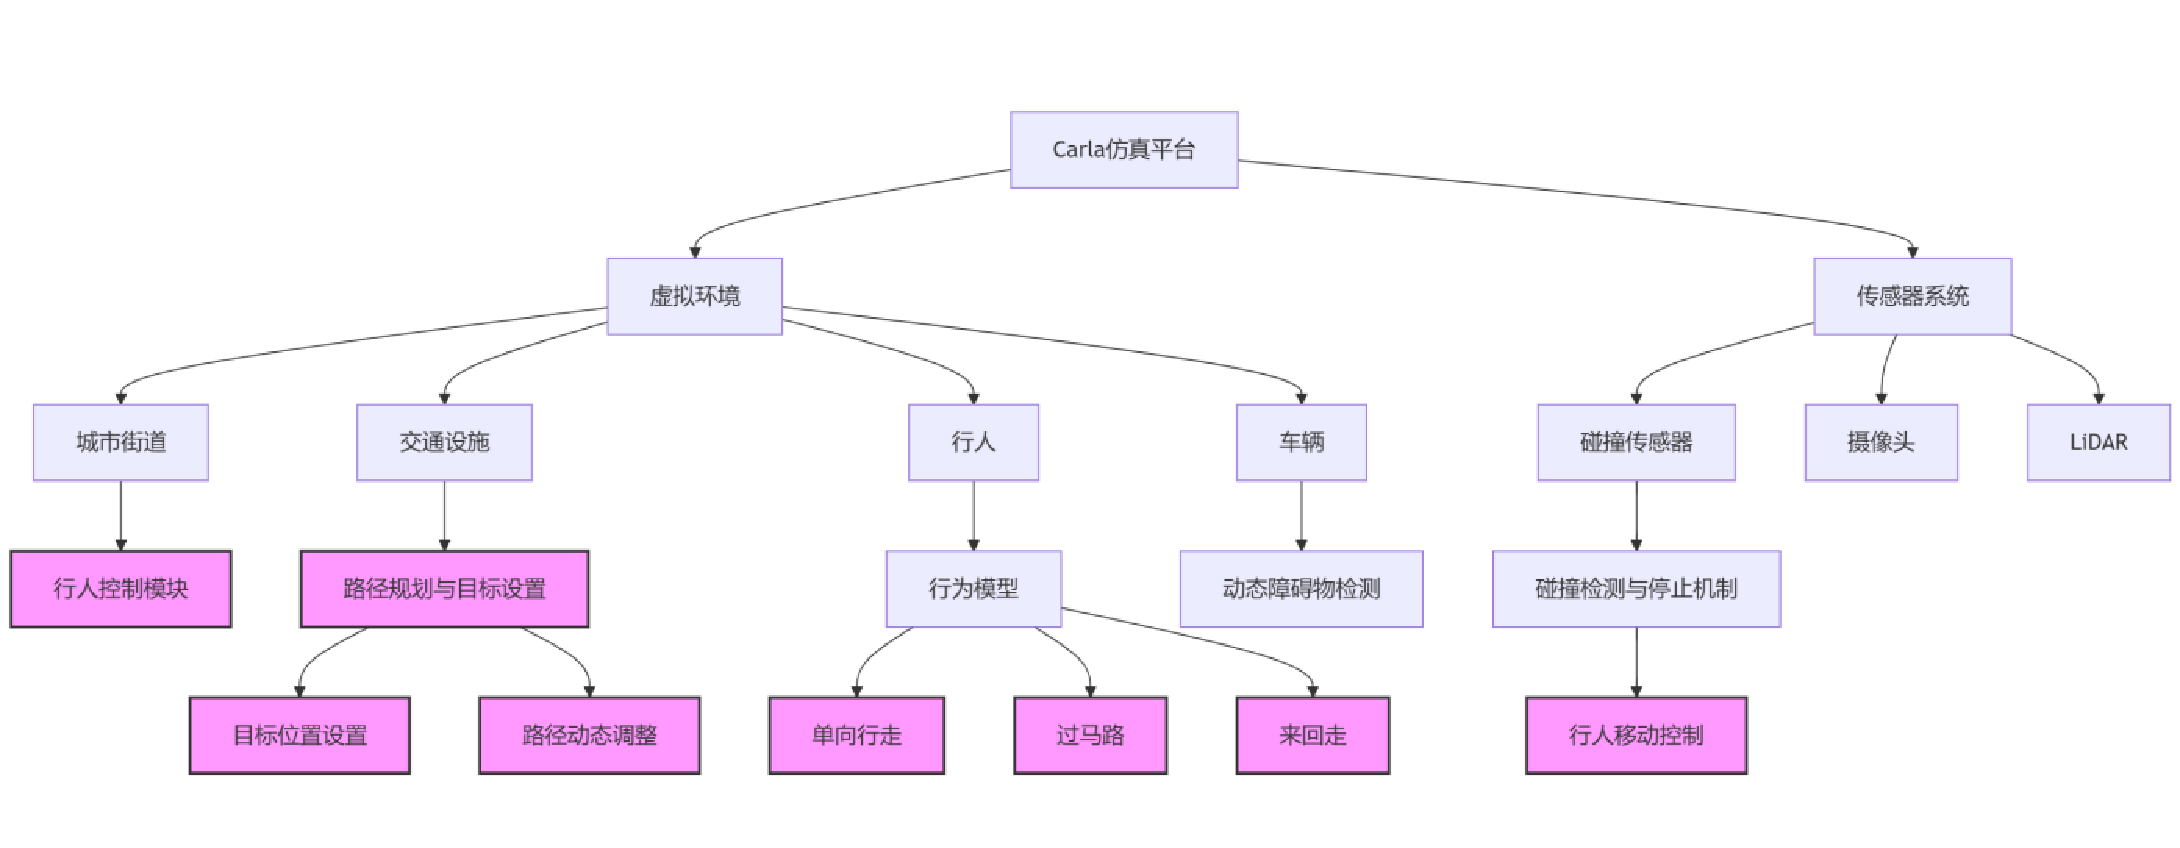
\includegraphics[width=0.8\textwidth]{images/system_architecture.pdf}
    \caption{行人控制系统架构示意图}
    \label{f.system_architecture}
\end{figure}

\section{行人骨骼控制}
在行人行为研究中,准确获取行人的骨骼姿态信息是实现行为理解与决策的关键环节。通过结合 Carla 平台的 AI 行人生成功能与自定义脚本设计,旨在将模拟环境中行人的骨骼数据完整采集、处理并用于后续的深度学习模型训练与验证。为了训练行人,必须确保它们不仅能够识别建筑物、道路和汽车,还能够识别人行道和过马路的行人,以确保行人以及其他动态障碍物的安全。Carla模拟器提供人工智能控制的行人,以人体形态填充模拟和训练数据。在许多计算机视觉应用中,人体姿态估计是一个重要因素,包括自动驾驶、安全、人群控制和多个机器人应用。 

Carla的API提供了从模拟中的行人获取真实骨架的功能。骨架由一组骨骼组成,每个骨骼都有一个根节点或顶点以及一个定义骨骼姿势(或方向)的向量。这些骨骼控制模拟行人的四肢和身体的运动。通过将各个骨骼的集合收集在一起,可以构建虚拟人姿势的模型,该模型可用于与神经网络估计的姿势模型进行比较,甚至用于训练神经网络进行姿势估计。通过使用 AI 控制器生成行人,恢复行人骨骼的真实三维坐标,并将这些骨骼投影到相机传感器捕获的二维图像上。使用这些的技术,在 Carla 模拟器为人体姿势估计框架设置训练和验证。通过保证骨骼数据采集的完整性和精度,为后续基于 Carla 环境的行人姿态估计与行为预测模型提供了坚实的数据基础。

\begin{figure}[H]
    \centering
    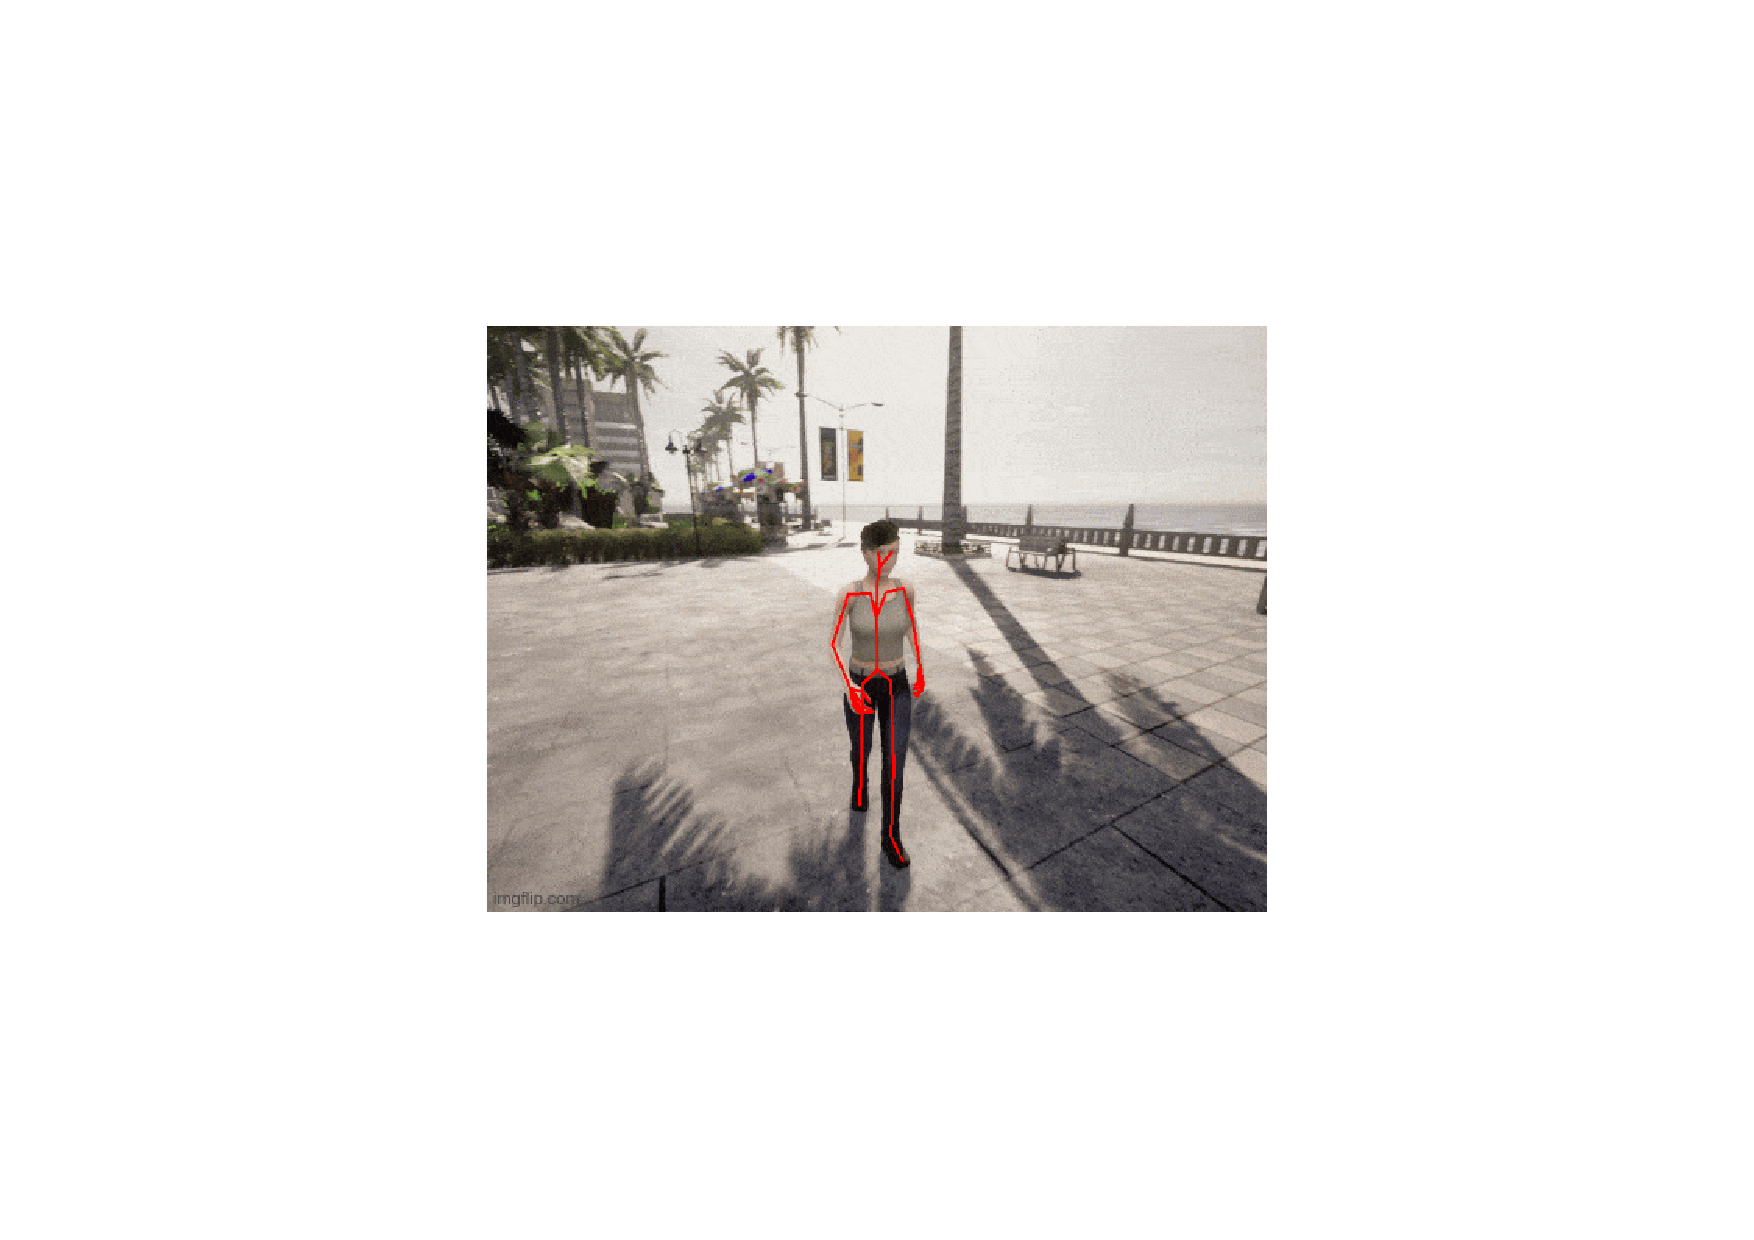
\includegraphics[width=0.8\textwidth]{images/pedestrian_skeleton.pdf}
    \caption{行人单向行走与过马路示意图}
    \label{f.pedestrian_skeleton}
\end{figure}

\section{行人行为控制}
本系统的行为控制模型建立在Carla平台提供的WalkerControl模块基础上,利用该模块能够精确地通过设定行人的方向和速度参数来操控其移动行为,使用的模拟地图为town5。除基本的移动功能外,系统还支持两种主要的行为模式:一是单向行走与过马路模式,二是来回走动模式。这些模式使得系统不仅能够在不同的场景中模拟行人的多样化行为,还可以满足后续复杂导航任务的需求。模块化设计与参数化配置,系统能够灵活适应不同实验需求,并为后续深度学习模型在行人避障与导航任务中的集成提供了稳定、高效的基础环境。在这一初步研究中并未加入动态障碍物,行人只是进行单独的行进,故具有局限性。

\subsection{单向行走与过马路}
单向行走与过马路是行人行为模式中最基础且至关重要的两个方面。行人在行走过程中通常从一个起点出发,遵循一条预先设定的路径,最终抵达目标位置。为了精确模拟行人过马路的行为,本研究设计了一个简易的路线规划系统,允许行人从街道的一侧安全地移动至对面。

实现过程为通过设定明确的目标位置,使行人能够沿着从起点到终点的预定路径行走。控制行人移动的核心在于使用Carla平台中的WalkerControl组件,该组件负责设定行人的位置、速度及其他运动参数。该模型较为简单,是本人初步探索calra行人行为模拟过程中的第一次实践。

\begin{figure}[H]
    \centering
    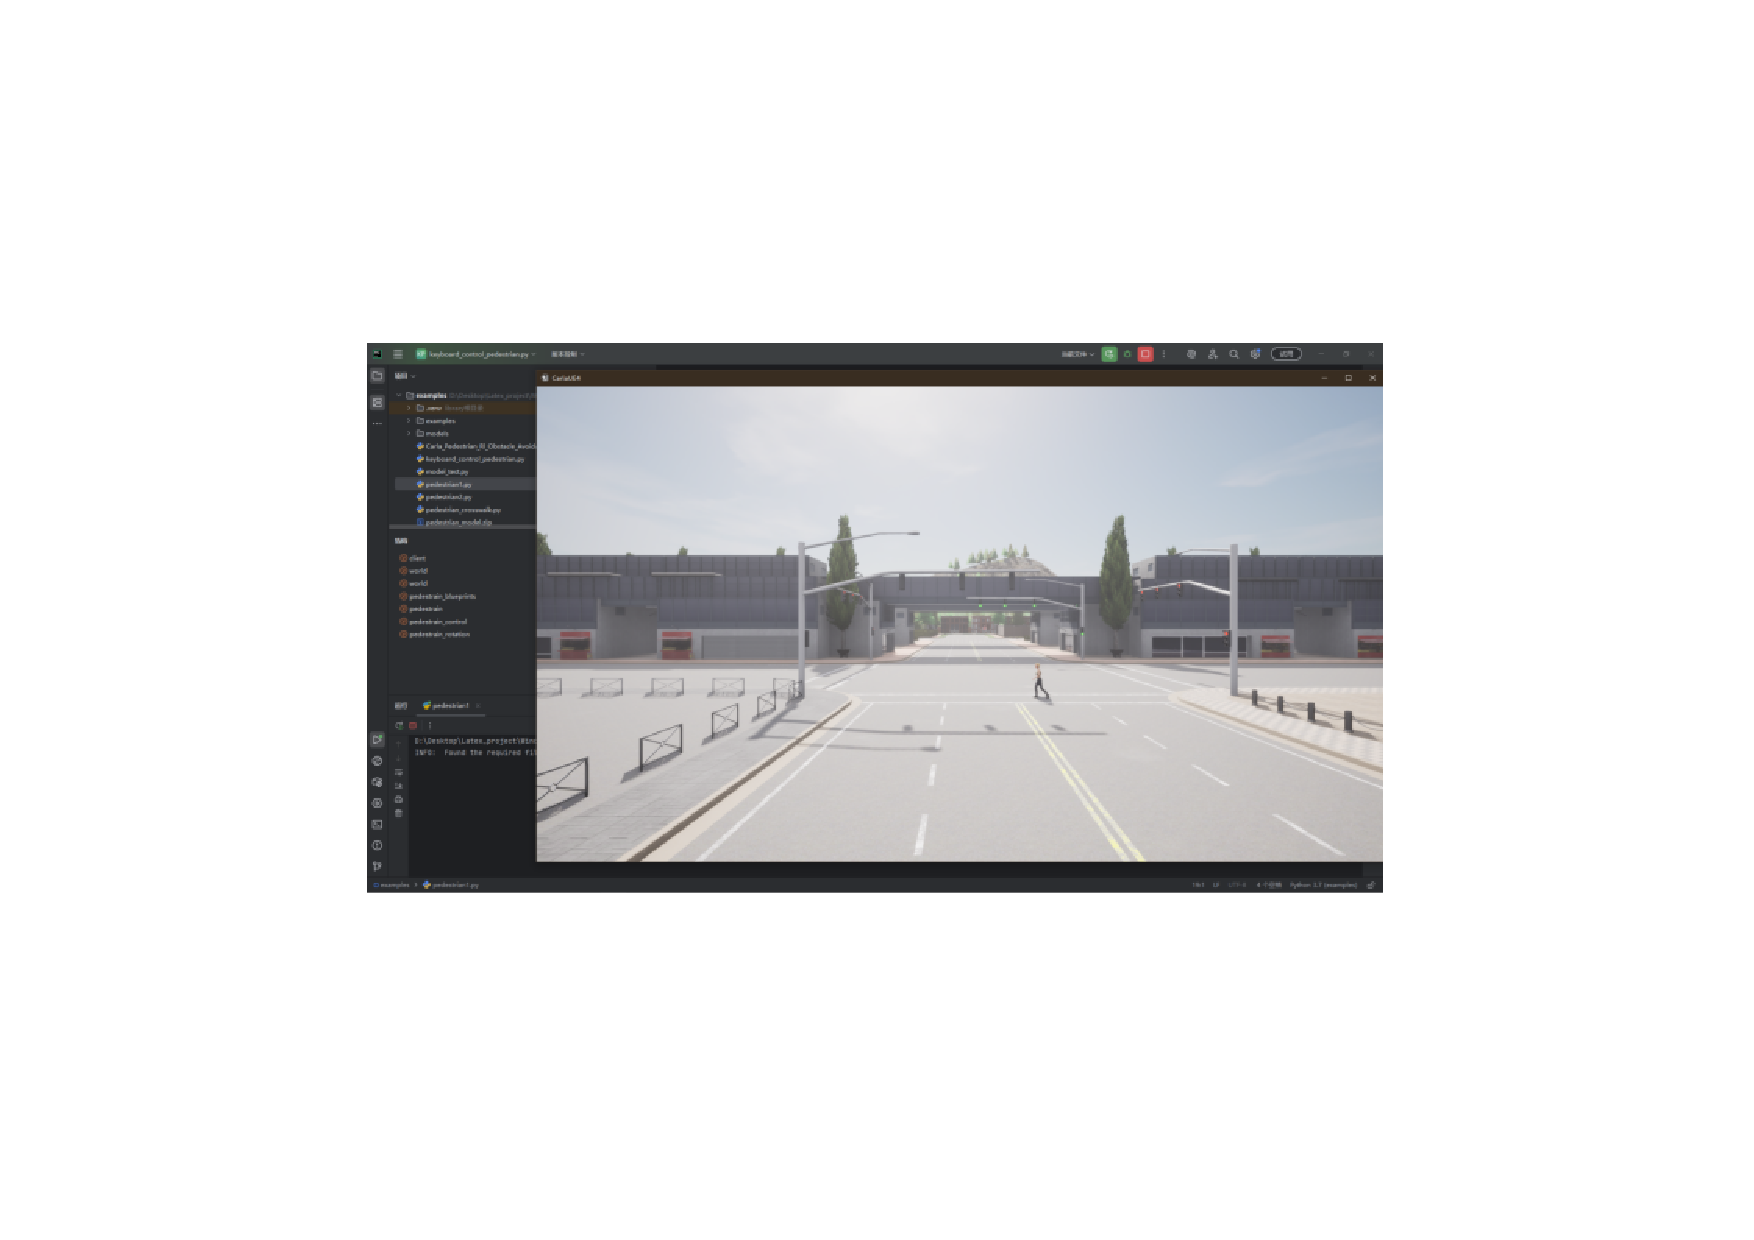
\includegraphics[width=0.8\textwidth]{images/crossing_path.pdf}
    \caption{行人单向行走与过马路示意图}
    \label{f.crossing_path}
\end{figure}

\subsection{来回走与路径控制}
在许多情况下,来回走动也是一种常见的行走模式,它使行人在两个固定点之间循环往复地行走。该行为模式特别适用于需要在短距离范围内反复行走的场景,比如本次模拟中的过马路过程。该模型的实现通过设定目标点并实时更新目标位置,从而确保行人能够按照既定路径高效地移动。

在实现过程中,目标点的设定首先通过指定两个目标位置来完成。行人到达一个目标位置后,系统会自动触发目标位置的改变,并使行人返回起点,完成来回走动的行为。该过程可以完全自动化进行,也可以根据应用场景的需求,允许行人通过手动操作来控制。为了使行人在运动过程中更加灵活地应对突发情况,遇到交通信号变化,系统会实时监测环境并调整行人动作,如遇到红灯则会原地等候,遇到绿灯直接通行。动态路径调整功能确保了行人能够根据实际情况及时作出反应,从而顺利到达下一个目标。这种智能路径规划技术不仅提高了行人行走效率,也增强了行走过程中的安全性,同时目标位置的设定也为后续的导航系统打下了基础。

\begin{figure}[H]
    \centering
    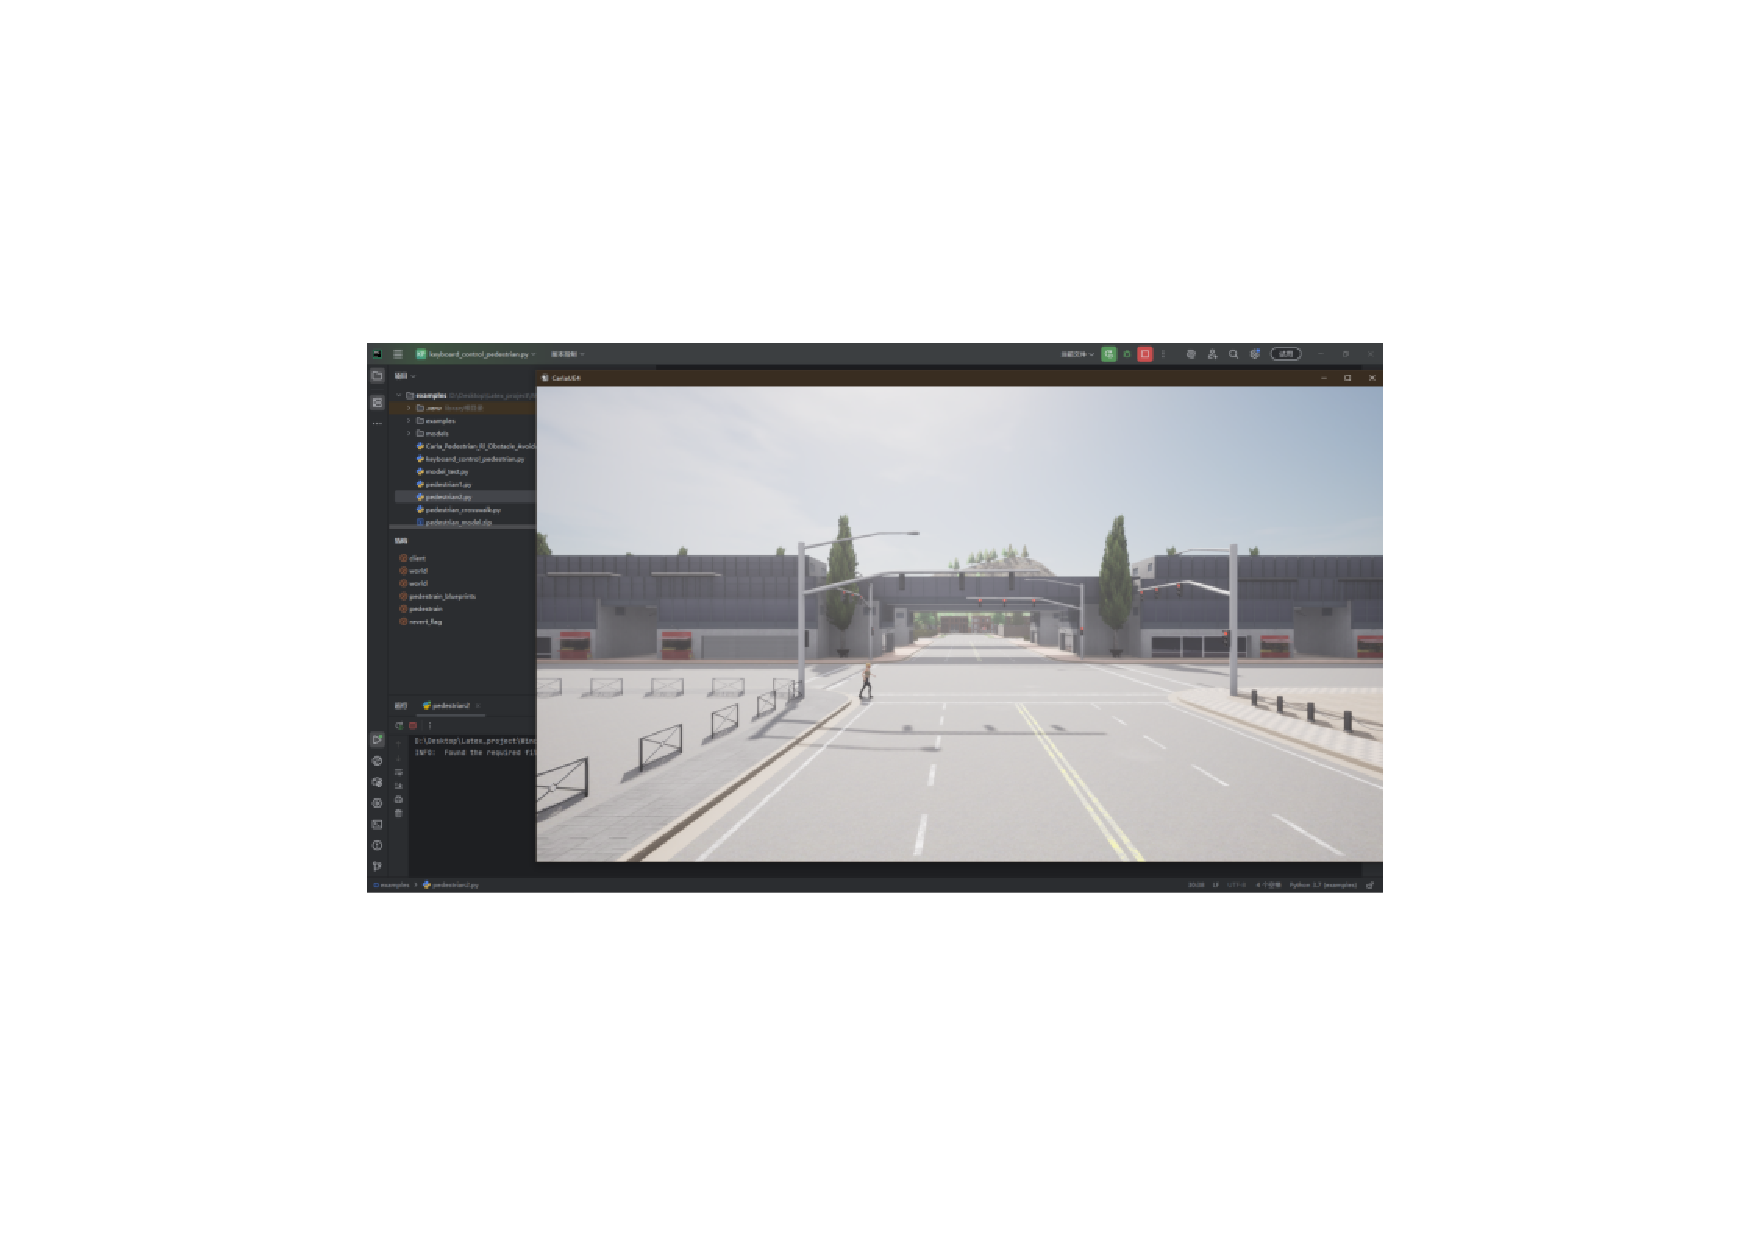
\includegraphics[width=0.8\textwidth]{images/walking_back_and_forth.pdf}
    \caption{行人来回走行为与来回过马路示意图}
    \label{f.walking_back_and_forth}
\end{figure}

\section{键盘控制行人移动}
为了进一步提升用户体验并增强系统的互动性,本研究也额外设计并实现了键盘控制功能,使用户能够通过简单的键盘输入直接操控行人的运动行为。同时采用了功能强大的Pygame库来监听键盘输入,使得用户通过按下特定按键(如W、A、S、D键)来实现对行人的前进、后退、转向等多样化动作控制。也在这一基础上,在Pygame库提供可视化框中提供了障碍物识别和监测功能,行人如果遇到障碍物,屏幕中会显示障碍物的距离等等一些实时反馈。

\begin{figure}[H]
    \centering
    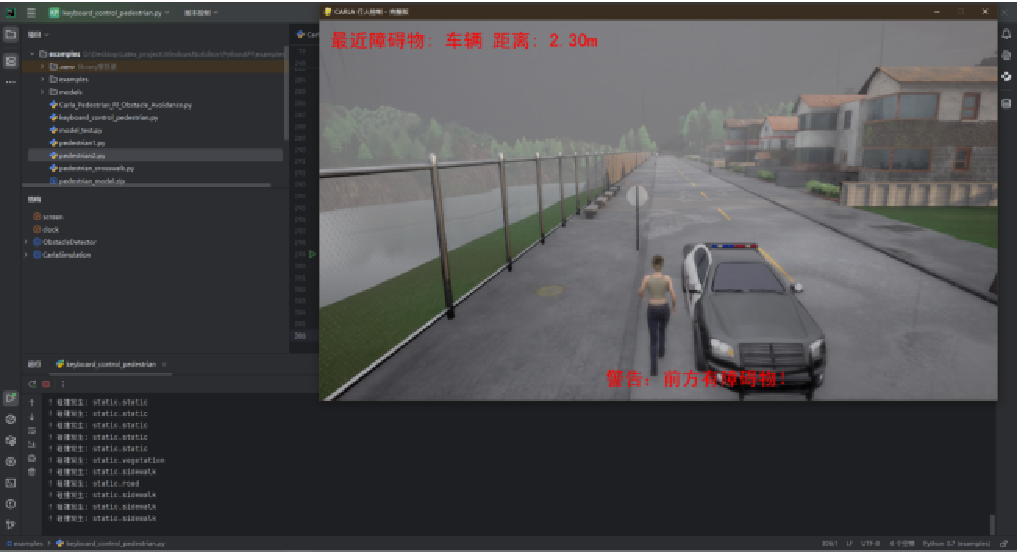
\includegraphics[width=0.8\textwidth]{images/collision_detection.pdf}
    \caption{行人障碍物检测示意图}
    \label{f.collision_detection}
\end{figure}

具体实现过程包括以下几个步骤:首先,通过Pygame库设置了键盘事件监听功能,使得系统能够捕捉到用户每一次的键盘操作,并将这些操作与行人运动方向精确映射。这样,用户通过键盘输入的每一指令都能被系统准确识别并执行。接着,设计控制逻辑,在用户输入指令后,行人的WalkerControl模块会实时响应并根据指令更新行人的方向和速度。这一过程确保了行人的移动能够即时且准确地反映用户的控制意图,从而实现了对行人运动的精确控制。最后,考虑到行人运动的安全性,系统加入了碰撞检测与停止机制。当行人在运动过程中遇到障碍物时,内置的碰撞传感器会立即检测到这一情况,并触发碰撞事件。接收到碰撞事件后,系统会迅速反应,立即停止行人的运动。这一措施有效避免了行人与障碍物发生碰撞的风险,从而保障了行人运动的安全性。

\begin{figure}[H]
    \centering
    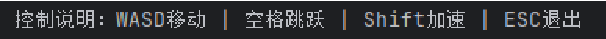
\includegraphics[width=0.8\textwidth]{images/keyboard_control.pdf}
    \caption{键盘控制行人规则}
    \label{f.keyboard_control}
\end{figure}

键盘控制模块不仅能实现对行人的灵活操控,也为调试与实验分析提供了完善的交互与可视化支持,为后续引入 AI 控制与自动化策略奠定基础。
